% Supplementary material: tables and figures that the main text summarizes.
% Build: latexmk -pdf supplement.tex
\documentclass[lettersize,journal]{IEEEtran}
\usepackage{amsmath,amsfonts}
\usepackage{array}
\usepackage{booktabs}
\usepackage{textcomp}
\usepackage{stfloats}
\usepackage{graphicx}
\usepackage{siunitx}
\graphicspath{{figures/}}
\sisetup{range-phrase={--}, range-units=single, per-mode=symbol}
\newcommand{\cA}{Circuit~A}
\newcommand{\cB}{Circuit~B}
\renewcommand{\thetable}{S\arabic{table}}
\renewcommand{\thefigure}{S\arabic{figure}}

\begin{document}

\title{Supplementary Material\\ Specification-Aware Fault Diagnosis of ECG Analog Front-Ends:
Bridging Alternate Test and Machine-Learning Diagnosis for In-Service Self-Test}
\author{Telmo~Miguel-Medina}
\maketitle

This document gives the tables and figures behind the results that the main text reports in
summary. Circuit~A is the front-end built around an integrated instrumentation amplifier and
Circuit~B the discrete three-op-amp front-end. Every number comes from the open dataset and code
of the article.

\section{Circuits and Measurements}

\begin{figure*}[!t]
\centering
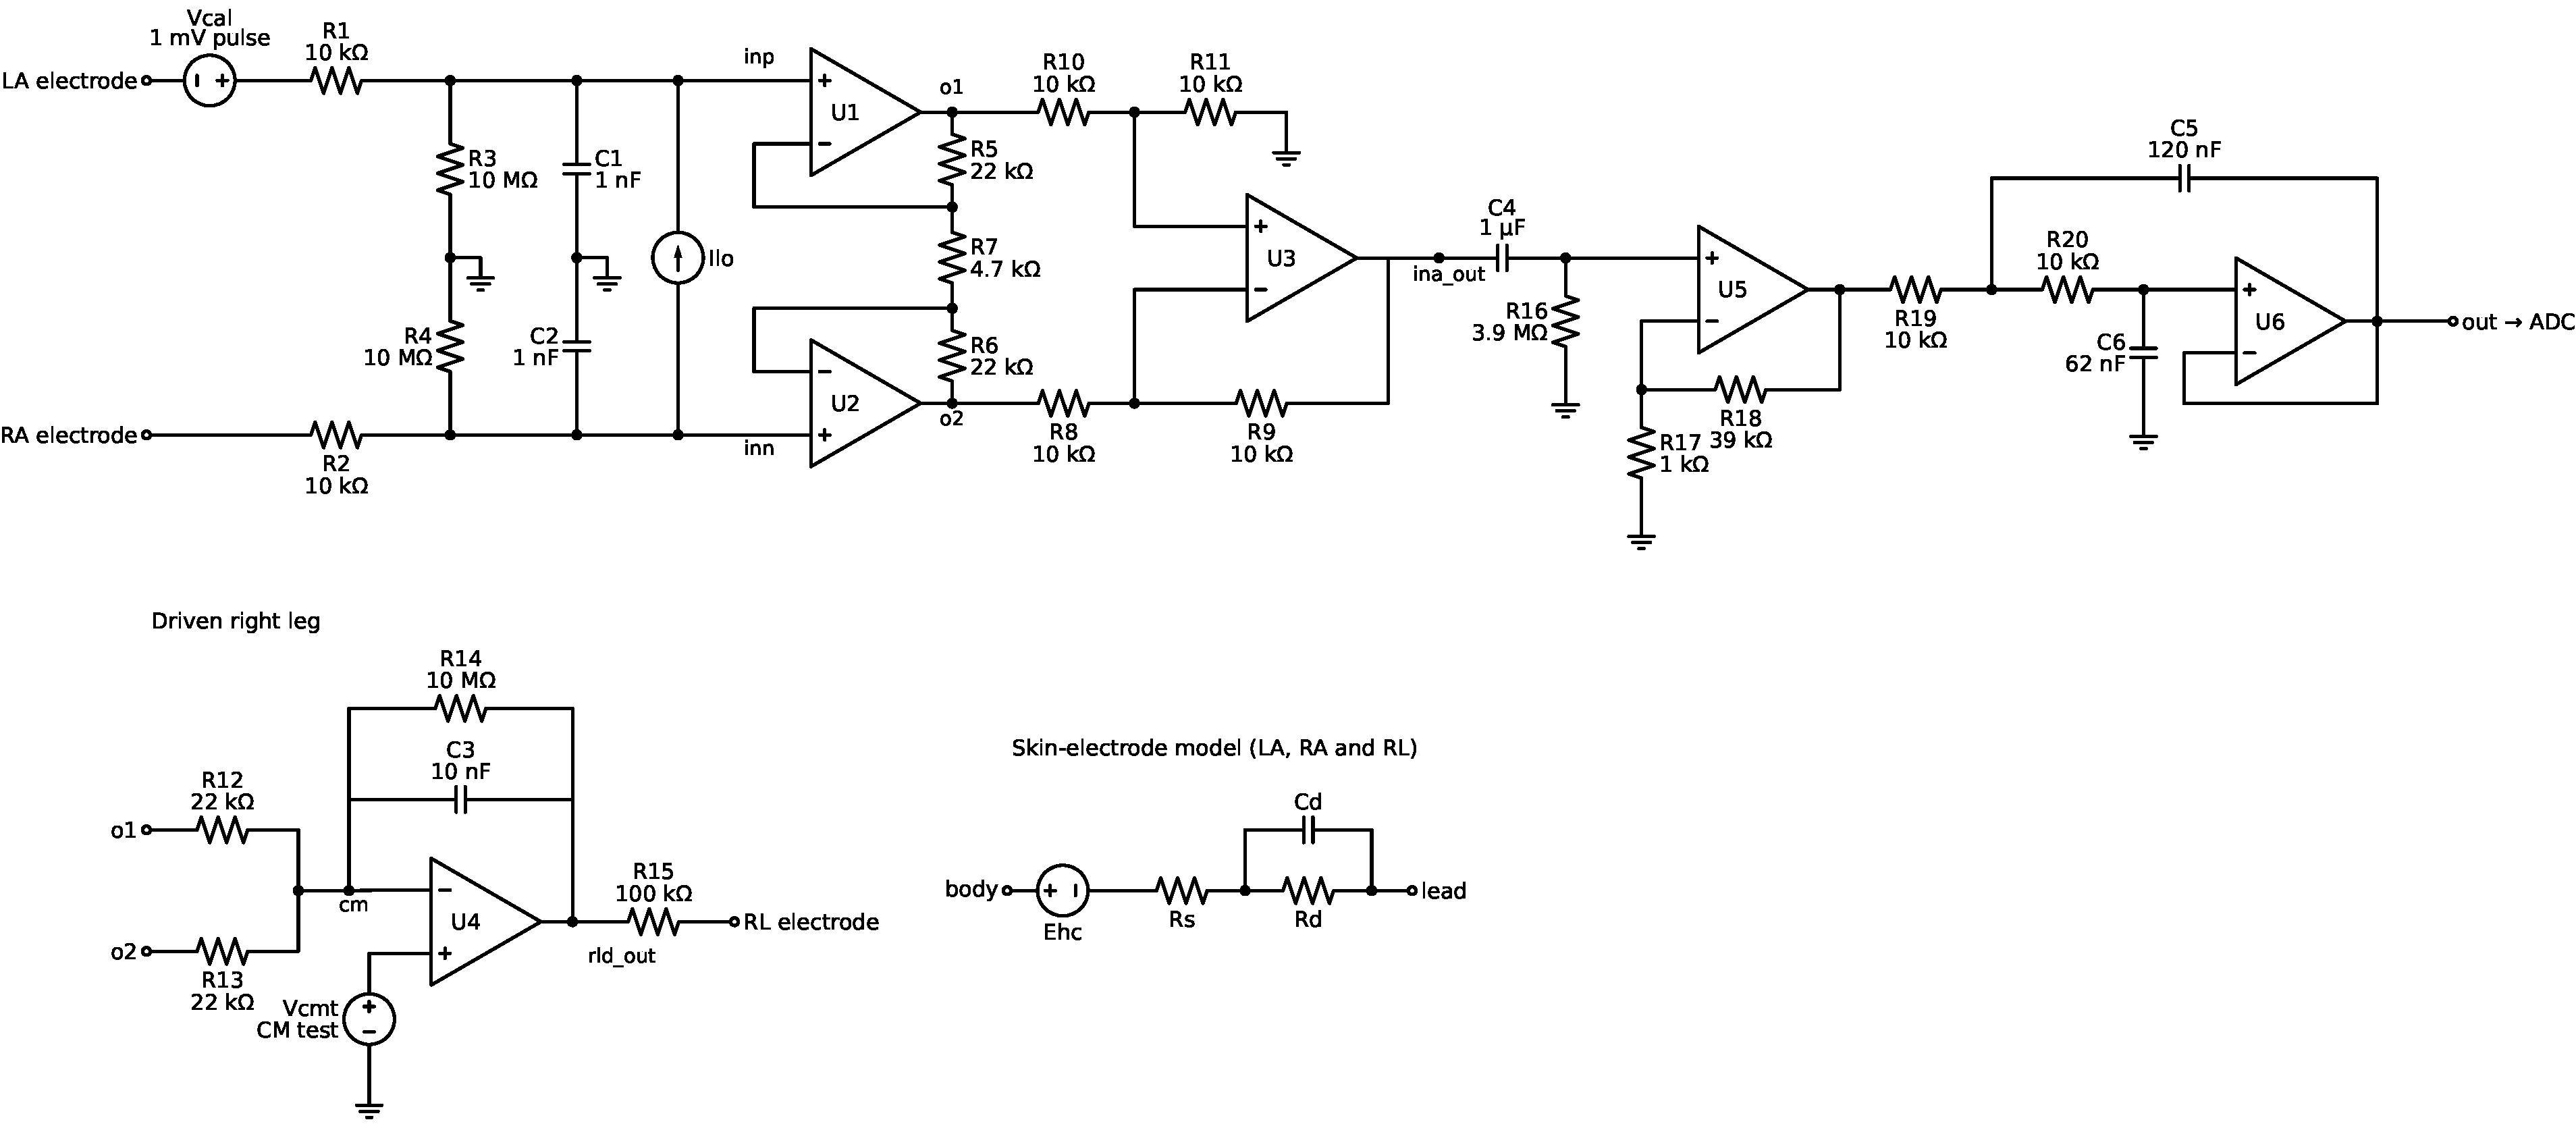
\includegraphics[width=\textwidth]{schematic_reference}
\caption{\cB: discrete three-op-amp instrumentation amplifier on $\pm$\SI{5}{\volt} supplies, with
the same filters, gain stage and driven-right-leg integrator as \cA.}
\end{figure*}

\begin{table}[!t]
\caption{The Two Circuits}
\label{tab:circuits}
\centering
\begin{tabular}{@{}lcc@{}}
\toprule
 & \cA & \cB \\
\midrule
Instrumentation amplifier & INA333 & three op-amps \\
Supply & \SI{3.3}{\volt} & $\pm$\SI{5}{\volt} \\
Gain (first stage / total) & 4.03 / 278 & 10.36 / 414 \\
Resistors / capacitors with faults & 16 / 8 & 20 / 6 \\
Discrete op-amps & 5 & 6 \\
Converter range & 0 to \SI{3.3}{\volt} & $\pm$\SI{2.5}{\volt} \\
Fault conditions & 293 & 307 \\
Simulated cases & \num{63600} & \num{66400} \\
\bottomrule
\end{tabular}
\end{table}

\begin{table}[!t]
\caption{Self-Test Measurements}
\label{tab:measurements}
\centering
\setlength{\tabcolsep}{3pt}
\begin{tabular}{@{}lp{0.58\columnwidth}cc@{}}
\toprule
Set & Measurement & Features & Time \\
\midrule
C1 & Dc level at the output and at the instrumentation-amplifier output & 2 & \SI{0.13}{\second} \\
C2 & Differential and common-mode tones at 0.05, 0.5, 10, 50 and \SI{150}{\hertz}: gain, phase and CMRR estimate & 15 & \SI{94}{\second} \\
C3 & Response to the \SI{1}{\milli\volt}, \SI{200}{\milli\second} calibration pulse: baseline, peak, final value, undershoot, tail, rise time, area & 7 & \SI{1}{\second} \\
C4 & Response to a \SI{1}{\nano\ampere} lead-off current at 10 and \SI{100}{\hertz} & 2 & \SI{2}{\second} \\
\bottomrule
\end{tabular}
\end{table}


\section{Functional Against Percentage Severity}
\begin{table}[!t]
\caption{Detector Trained on the Percentage Label or on the Functional Label, Scored Against
Compliance. Mean of Three Repetitions, in Percent}
\label{tab:severity}
\centering
\begin{tabular}{@{}llccc@{}}
\toprule
Circuit & Trained on & Labeled bad & Escapes & False rejects \\
\midrule
A & Percentage & 88.7 & 7.9 & 36.8 \\
 & Functional & 21.0 & 4.1 & 1.6 \\
B & Percentage & 89.2 & 8.3 & 36.5 \\
 & Functional & 30.2 & 7.6 & 2.2 \\
\bottomrule
\end{tabular}
\end{table}


\section{Location and Origin}
\begin{table}[!t]
\caption{Location of the Cause on Non-Compliant Cases: Macro F1 (Mean of Three Repetitions)}
\label{tab:location}
\centering
\begin{tabular}{@{}lcccc@{}}
\toprule
 & \multicolumn{2}{c}{By ambiguity group} & \multicolumn{2}{c}{By component} \\
\cmidrule(lr){2-3}\cmidrule(l){4-5}
Model & A & B & A & B \\
\midrule
$k$-nearest neighbors & 0.83 & 0.70 & 0.67 & 0.55 \\
Random forest & 0.86 & 0.76 & 0.74 & 0.61 \\
Support vector machine & 0.86 & 0.71 & 0.69 & 0.53 \\
Gradient boosting & 0.87 & 0.74 & 0.73 & 0.59 \\
Multilayer perceptron & 0.81 & 0.71 & 0.66 & 0.53 \\
Convolutional network$^{\mathrm{a}}$ & 0.56 & 0.32 & -- & -- \\
\bottomrule
\multicolumn{5}{@{}l}{\footnotesize $^{\mathrm{a}}$On the sampled pulse response only.}
\end{tabular}
\end{table}

\begin{table}[!t]
\caption{Origin Classification on the Test Part of One Repetition (Random Forest, Main Feature
Set)}
\label{tab:origin}
\centering
\begin{tabular}{@{}llcccc@{}}
\toprule
 & & \multicolumn{3}{c}{Predicted} & \\
\cmidrule(lr){3-5}
Circuit & True & None & Circuit & Electrode & Recall \\
\midrule
A & None & \num{14314} & 63 & 60 & \SI{99.2}{\percent} \\
 & Circuit & 189 & \num{3649} & 25 & \SI{94.5}{\percent} \\
 & Electrode & 269 & 15 & 496 & \SI{63.6}{\percent} \\
\addlinespace
B & None & \num{13029} & 136 & 68 & \SI{98.5}{\percent} \\
 & Circuit & 445 & \num{5417} & 45 & \SI{91.7}{\percent} \\
 & Electrode & 278 & 25 & 477 & \SI{61.2}{\percent} \\
\bottomrule
\end{tabular}
\end{table}


\begin{figure}[!t]
\centering
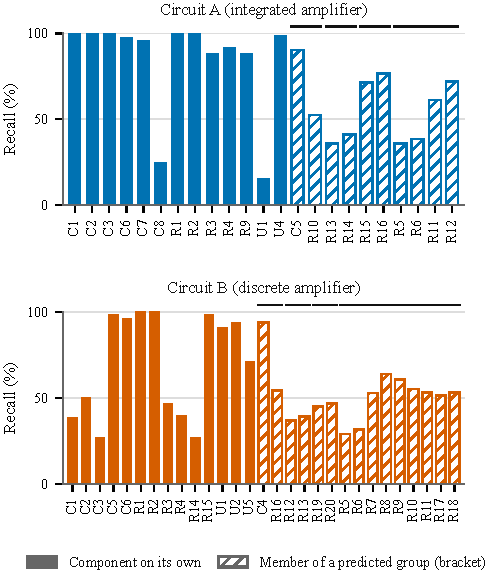
\includegraphics[width=\columnwidth]{recall_by_component}
\caption{Recall of each component by the best component-level model (random forest) on
non-compliant cases. Hatched bars are members of the ambiguity groups predicted from the
sensitivities of the nominal circuit; a bracket joins the members of each group.}
\end{figure}

\section{Robustness and Minimal Set of Measurements}
\begin{table}[!t]
\caption{Robustness of the Compliance Decision (Class-Weighted Classifier) and of Group-Level
Location. Mean of Three Repetitions}
\label{tab:robustness}
\centering
\setlength{\tabcolsep}{3pt}
\begin{tabular}{@{}p{0.40\columnwidth}cccccc@{}}
\toprule
 & \multicolumn{3}{c}{\cA} & \multicolumn{3}{c}{\cB} \\
\cmidrule(lr){2-4}\cmidrule(l){5-7}
Condition & Esc. & F.r. & F1 & Esc. & F.r. & F1 \\
\midrule
Default (\SI{1}{\milli\volt}, 12 bits) & 4.1 & 1.7 & 0.88 & 7.6 & 2.2 & 0.77 \\
\SI{10}{\milli\volt} noise, matched training & 4.2 & 1.6 & 0.86 & 7.8 & 2.2 & 0.75 \\
\SI{10}{\milli\volt} noise, trained at \SI{1}{\milli\volt} & 9.7 & 1.2 & 0.79 & 6.6 & 18.8 & 0.71 \\
8 bits, matched training & 3.9 & 1.6 & 0.88 & 7.5 & 2.2 & 0.76 \\
8 bits, trained at 12 bits & 7.0 & 1.2 & 0.87 & 7.2 & 4.2 & 0.75 \\
Truncated Gaussian tolerances & 3.8 & 1.6 & 0.89 & 7.4 & 2.4 & 0.77 \\
\SI{2}{\percent} resistors, \SI{10}{\percent} capacitors & 7.1 & 1.9 & 0.87 & 11.4 & 2.9 & 0.45 \\
\bottomrule
\multicolumn{7}{@{}p{0.97\columnwidth}@{}}{\footnotesize Esc.: escapes (\%). F.r.: false rejects
(\%). F1: macro F1 of the location by ambiguity group. The last two rows are scored on
separately generated datasets.}
\end{tabular}
\end{table}


\begin{figure*}[!t]
\centering
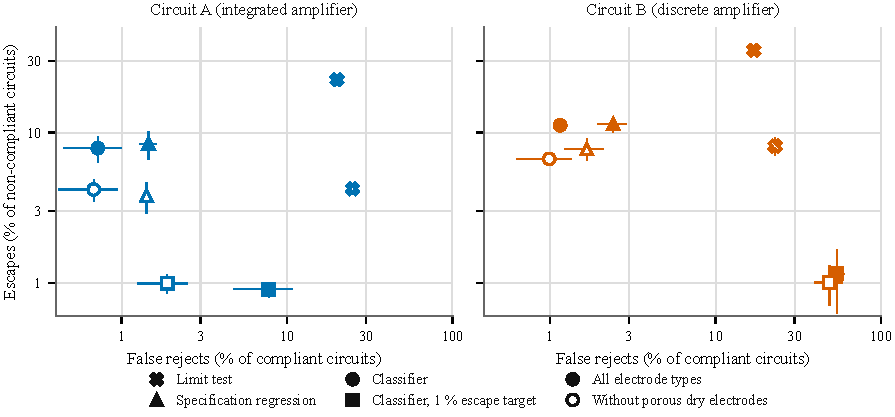
\includegraphics[width=\textwidth]{operating_points_full}
\caption{Operating points of the four decision methods with \SI{95}{\percent} confidence
intervals over three repetitions, for all electrode types (filled markers) and without porous dry
electrodes (open markers).}
\end{figure*}

\begin{figure*}[!t]
\centering
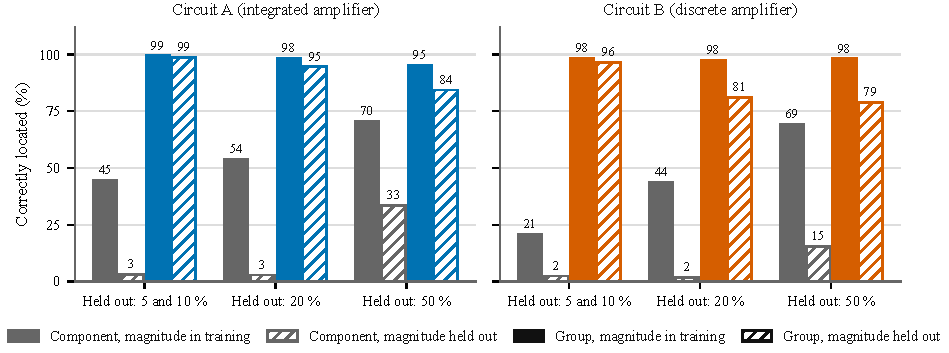
\includegraphics[width=\textwidth]{unseen_magnitudes_full}
\caption{Location of the cause for parametric faults of magnitudes present in training or held
out of it, scored on the non-compliant cases of those magnitudes.}
\end{figure*}

\begin{figure*}[!t]
\centering
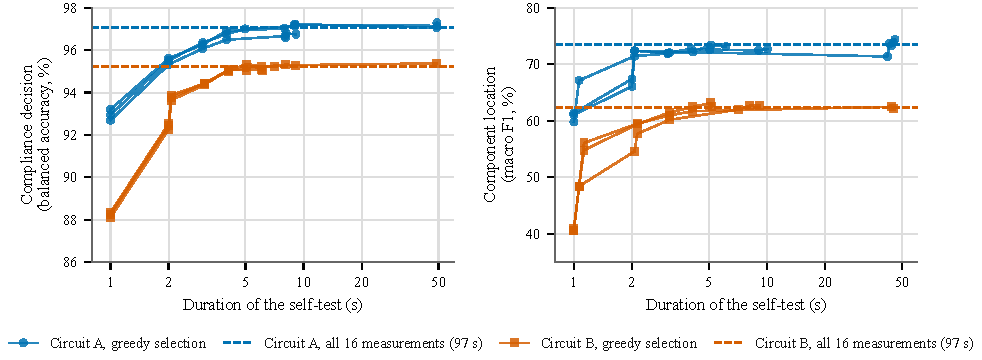
\includegraphics[width=\textwidth]{cost_performance_full}
\caption{Score on the test part as self-test measurements are added one at a time by greedy
selection, for the compliance decision and for component location. One line per repetition;
dashed lines are the score with all the measurements.}
\end{figure*}

\end{document}
